\chapter{Navržené řešení}
\label{sec:Propesed_solution}

Velká většina výzkumných prací, které se počítáním lidí v obraze zabývají, se snaží jejich množství určit na základě jediného snímku.
Toto je celkem logicky dáno jednodušší dostupností anotovaných datasetů, které jsou v případě, že se jedná pouze o jednotlivé snímky a ne videosekvence, mnohem obsáhlejší a zachycují mnohem větší množství nejrůznějších situací z mnoha úhlů pohledu.
Temporální informace ale mohou být při počítání objektů v obraze velmi cennou informací, kterou by neuronová síť mohla využít pro snazší řešení situací, kdy jsou lidé v obraze zakryti jinými lidmi či objekty, a zlepšit tak přesnost výsledného počtu.
Je totiž velmi nepravděpodobné, že člověk procházející zachycovanou scénou mezi dvěma po sobě jdoucími snímky zničehonic ze scény zmizí.
Je samozřejmě možné, že tento člověk například zašel za roh, nebo byl zakryt kolem projíždějící dodávkou, ale pokud je stále alespoň trochu patrné, že se v obraze nachází a je překryt pouze částečně, tak by měl být do výsledného počtu rozhodně započítán. Pokud by taková situace byla vyhodnocována pouze na základě jediného snímku, tak by nepochybně bylo přesné spočítání lidí obtížné i pro člověka. Předchozí snímky přitom často obsahují informace, které by při rozhodování, zda se opravdu jedná o člověka, mohly výrazně pomoci.

\begin{figure}[h!]
	\centering
	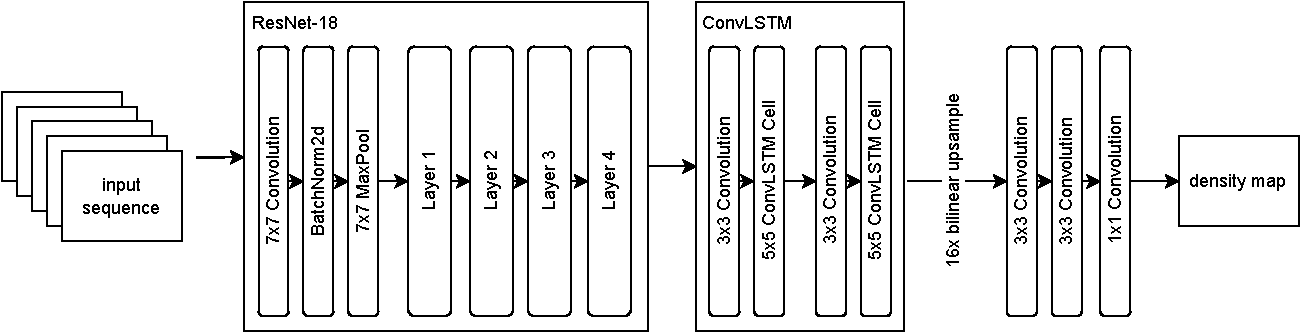
\includegraphics[width=\textwidth]{Figures/solution/net_structure.pdf}
	\caption{Struktura navržené sítě}
	\label{fig:proposed_net}
\end{figure}

Neuronová sít navržená v této práci se tohoto snaží využít a jejím cílem je vytvořit ze vstupní sekvence \(n\) po sobě jdoucích snímků vytvořit dvoudimenzionální hustotní mapu, která vyobrazuje hustotu výskytu lidí v posledním snímku vstupní sekvence, a suma jejíž pixelů bude rovna celkovému počtu lidí v něm. Na obrázku \ref{fig:proposed_net} je vyobrazena struktura stíě navržené v této práci.
Jak je z obrázku patrné, tak se skládá z několika částí, které budou v této kapitole blíže popsány.

\section{ResNet}
Residuální neuronová síť (ResNet) \cite{ResNet} byla poprvé představena v roce 2015, kdy vyhrála ImageNet Large Scale Visual Recognition Challenge, a svou architekturou silně ovlivnila budoucnost návrhu neuronových sítí.
Síla této neuronové sítě spočívá v tom, že přináší způsob, jak snížit vliv tzv. problému mizejícího gradientu (vanishing gradient problem).
Komplexita neuronových sítí se s každým rokem zvyšuje. Nejvíce se ale konvoluční neuronové sítě rozrůstají do hloubky. Čím je totiž neuronová síť hlubší, tím komplexnější příznaky dokáže extrahovat z původního vstupu a tím složitější funkce dokáže aproximovat.
Čím je ale neuronová síť hlubší, tím více se projevuje problém mizejícího gradientu.
Když je při trénování sítí šířena chyba pomocí algoritmu backpropagation, dochází k tomu, že její vliv je na svrchních vrstvách menší, než na hlubokých. Je-li tedy síť příliš hluboká, tak gradient je na svrchních vrstvách tak malý, že nedochází k přenastavení vah a tyto vrstvy se tedy nijak nemění.
Prohloubení sítě tedy v tomto případě ztrácí smysl a dokonce může mít negativní vliv na její výsledky.
Mělčí neuronové sítě proto mohou při řešení stejného problému dosáhnout mnohem lepších výsledků.

\begin{figure}[h!]
	\centering
	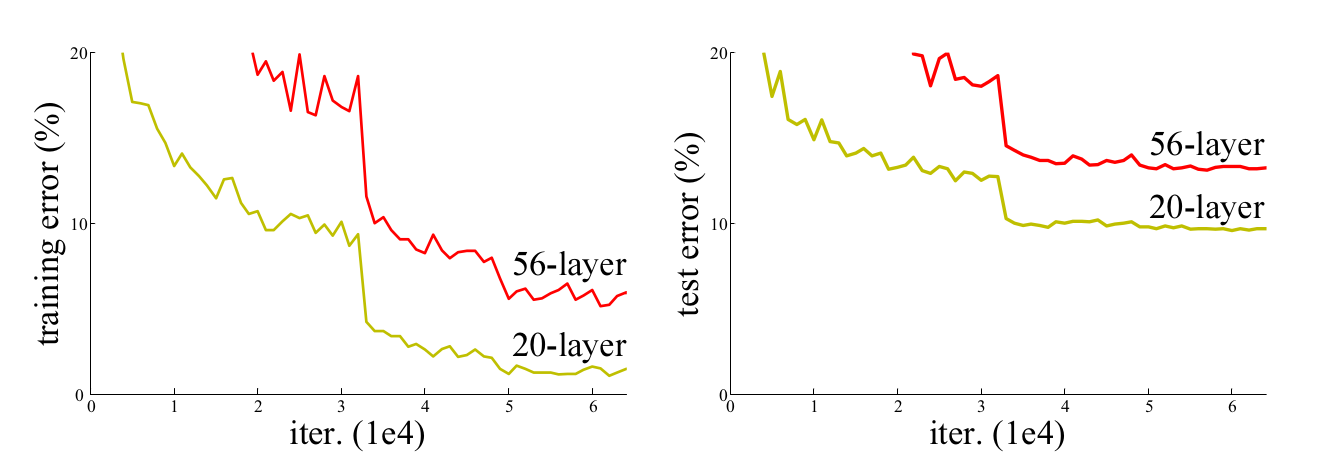
\includegraphics[width=0.7\textwidth]{Figures/solution/vanishing_gradient.png}
	\caption{Porovnání chyby při testování a trénování dvou sítí o hloubce 20 a 56 vrstev určených ke klasifikaci na datasetu CIFAR-10 \cite{ResNet}}
\end{figure}

Síť ResNet je tvořena reziduálními bloky, které jsou podobné VGG blokům \cite{VGG}.
Každý blok obsahuje dvě konvoluce o velikosti 3x3 a každá konvoluce je následovaná normalizací dávky (batch normalization) a aktivační funkcí ReLU.
Co ale reziduální blok přidává je tzv. zkratkové spojení (shortcut connection), které právě pomáhá snižovat vliv mizejícího gradientu.
Zkratkové spojení vezme vstupní hodnoty reziduálního bloku a přidá je k hodnotám před spuštěním druhé aktivační funkce.
V praxi to znamená, že vstupní hodnoty prochází v bloku dvěma cestami, kdy v jedné jsou změněny dvěma konvolucemi, zatímco v druhé se těmto konvolucím vyhnou. Při zpětném šíření chyby sítí se tedy chyba dostane do horních vrstev mnohem rychleji, takže navrhovaná síť může být mnohem hlubší.

\begin{figure}[h!]
	\centering
	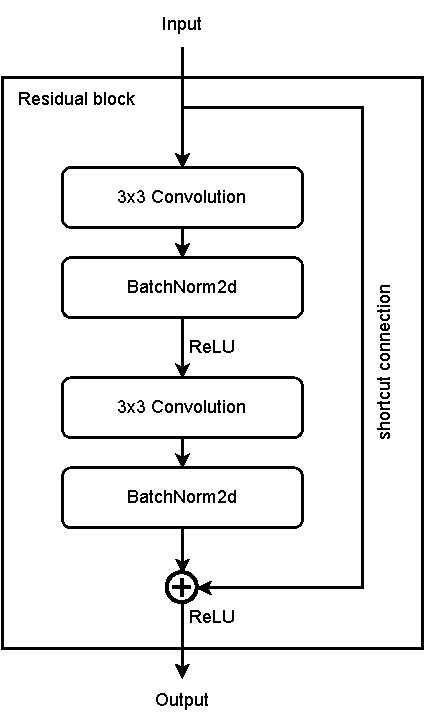
\includegraphics[width=0.3\textwidth]{Figures/solution/residual_block.pdf}
	\caption{struktura reziduálního bloku}
	\label{fig:residual_block}
\end{figure}

Síť ResNet je v navržené síti použita hned na vstupu a jejím cílem je zredukovat dimenzi vstupní sekvence po sobě jdoucích snímků a extrahovat z jednotlivých snímků důležité příznaky, které následně budou využity pro extrakci temporálních informací a konstrukci výsledné hustotní mapy.
Konkrétně je použita síť ResNet18, která obsahuje pouze čtyři reziduální bloky.
Tato varianta byla zvolena kvůli omezenému množství paměti na testovacím stroji.

\section{ConvLSTM}
Tradiční konvoluční neuronové sítě jsou výborným nástrojem pro zjišťování a práci s příznaky v prostorové doméně. Pokud je ale potřeba kromě prostorových dat nutné pracovat i s temporálními informacemi, musíme použít jiný nástroj. V takovém případě se nabízí použití ConvLSTM (Convolutional Long Short-Term Memory) sítě. Ta byla poprvé představena v roce 2015 v článku \cite{ConvLSTM}. Pro pochopení, jak ConvLSTM funguje, je ale nejdříve důležité pochopit, na jakém principu funguje tradiční LSTM síť, na které je ConvLSTM založená.

LSTM patří do skupiny rekurentních neuronových sítí (RNN), které slouží ke zpracování sekvenčních dat, kde existuje závislost aktuálního vstupu na předchozím.
Problémem použití klasických neuronový sítí na taková data je, že neuronová síť řeší každý vstup zvlášť a nemá žádný mechanismus, pomocí kterého by si dokázal spojit předchozí vstupy s těmi aktuálními.
Samozřejmě by se nabízela možnost dát na vstup neuronové sítě celou vstupní sekvenci, nebo alespoň její část, která se nachází bezprostředně před aktuálním vstupem, avšak to by znamenalo, že výsledná neuronová síť by musela být mnohem komplexnější, což by znamenalo větší nároky na výpočetní sílu a velikost trénovací množiny.
Rekurentní neuronové sítě tento problém řeší tím, že přidávají stavové proměnné, které ukládají informace o předchozích vstupech a jsou zpracovávány společně s aktuálním vstupem.

\begin{figure}[h!]
	\centering
	\subfloat[Architektura RNN]{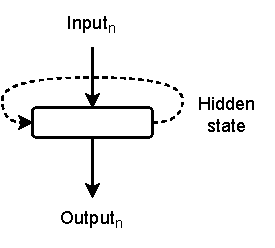
\includegraphics[width=0.3\textwidth]{Figures/solution/RNN_architecture.pdf}}
	\subfloat[Architektura RNN (rozvinutá)]{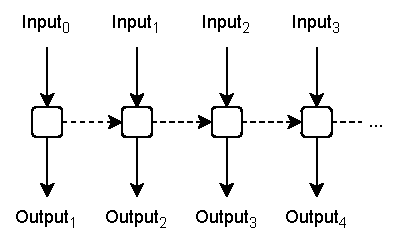
\includegraphics[width=0.4\textwidth]{Figures/solution/RNN_architecture_unrolled.pdf}}
	\caption{Diagram architektury RNN}
	\label{fig:RNN_architecture}
\end{figure}

Jak je patrné z obrázku \ref{fig:RNN_architecture}, tak pro každý vstup ve zpracovávané sekvenci je na základě tohoto vstupu a stavu stavové proměnné vzniklé zpracováním předchozího vstupu vytvořen výstup a nový stav skryté proměnné.
Jelikož je tato skrytá proměnná každým aktuálním vstupem měněna, dochází k tomu, že informace, která do ní byla zapsána při zpracování starších vstupů, ztrácí na významu a je překryta novějšími vstupy.
Rekurentní neuronové sítě z tohoto důvodu trpí problémy s dlouhodobější pamětí a jejich paměť je spíše krátkodobá.

LSTM se tento problém snaží vyřešit tak, že je specificky designovaná tak, aby více udržovala i dlouhodobější informace \cite{understaning_lstm}.
Samotný koncept LSTM již je celkem starý.
Poprvé byla síť LSTM představena v roce 1997 Hochreiterem a Schmidhuberem \cite{LSTM}.
Schéma LSTM je zobrazeno na obrázku \ref{fig:LSTM_architecture} a mnohým může připomínat strukturu logického obvodu.
Od toho se odvíjí i názvosloví, které tuto problematiku obklopuje, jelikož často mluví o branách.
Jak může být ze schématu patrné, tak LSTM má dvě stavové proměnné.

\begin{figure}[h!]
	\centering
	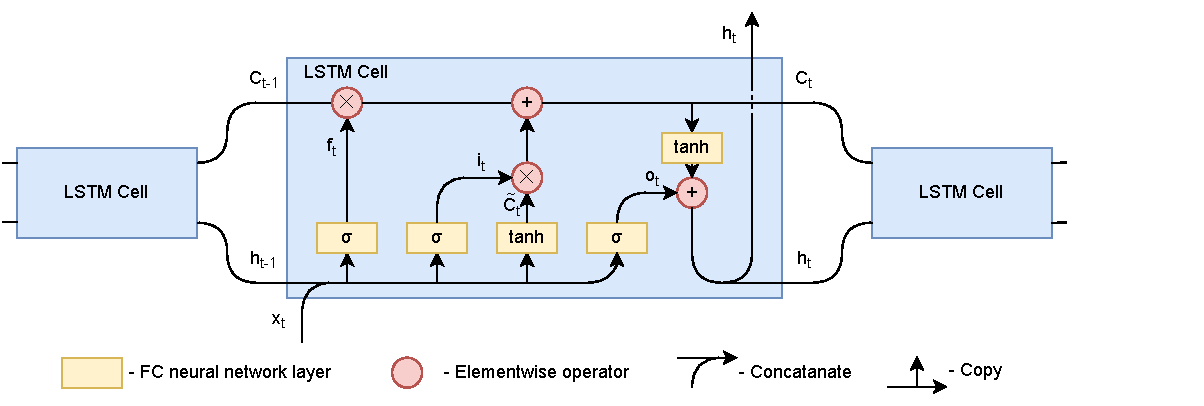
\includegraphics[width=\textwidth]{Figures/solution/LSTM_diagram.pdf}
	\caption{Struktura LSTM}
	\label{fig:LSTM_architecture}
\end{figure}



První z nich (procházející vrchní částí diagramu) slouží k ukládání dlouhodobých informací a často se nazývá stav buňky (cell state). Druhá z nich se nazývá skrytý stav (hidden state) a jedná se o paměť, se kterou LSTM buňka aktivně pracuje a na základě které rozhoduje, jak postupovat dále.
Postup vyhodnocování vstupních informací se dá rozdělit do několika kroků.

\begin{enumerate}

\item Na základě informací, které jsou obsaženy ve skrytém stavu a vstupním vektoru, je rozhodnuto, jaké informace ze stavu buňky budou ponechány a jaké budou zapomenuty.
O toto se stará tzv. zapomínací brána (Forget gate), tvořená plně propojenou vrstvou se sigmoidální aktivační funkcí.
Tato brána je následována Hadamardovým součinem výsledku této operace se stavem buňky.

Má-li být informace uložená v daném prvku stavu buňky zapomenuta, nastaví plně propojená vrstva hodnotu v odpovídajícím prvku na nulu.
V případě, že má být informace v prvku ponechána tak, jak je, bude ve výsledku FC vrstvy jednička.
Výsledek FC vrstvy samozřejmě může být jakékoliv číslo v intervalu \(<0;1>\) v závislosti na tom, jak moc má být informace zapomenuta a její vliv na další výpočet snížen.
Tuto bránu lze vyjádřit rovnicí \ref{eq:forget_gate}. 

\begin{equation}
f_t = \sigma(W_f \cdot [h_{t-1}, x_t] + b_f)
\label{eq:forget_gate}
\end{equation}


\item Následuje rozhodnutí o tom, jaké nové informace mají být ve stavu buňky uloženy.
Podobně jako v předchozím kroce jsou vstupní data společně se skrytým stavem dána na vstup vstupní brány (Input gate) tvořené FC vrstvou se sigmoidální aktivační funkcí, která určuje, jaká data mají být zapamatována.

\begin{equation}
i_t = \sigma(W_i \cdot [h_{t-1}, x_t] + b_i)
\label{eq:input gate}
\end{equation}

Než jsou ale data do stavu buňky přidána, jsou předtím zpracována vstupní modulační branou (Input Modulation gate), která je také tvořena FC vrstvou, ale používá jako aktivační funkci hyperbolický tangens (\(\tanh\)).
Výsledek této operace je po složkách vynásoben s výsledkem vstupní brány a tento násobek je opět po jednotlivých složkách přičten k patřičným složkám ve stavu buňky.

\begin{equation}
\widetilde{C}_t = \tanh(W_{\widetilde{C}} \cdot [h_{t-1}, x_t] + b_{\widetilde{C}})
\label{eq:input_modulation_gate}
\end{equation}

Tímto jsou ukončeny veškeré modifikace stavu buňky \(C_t\) které by se daly vyjádřit rovnicí \ref{eq:cell_state_modification}.

\begin{equation}
C_t = f_t * C_{t-1} + i_t * \widetilde{C}_t
\label{eq:cell_state_modification}
\end{equation}



\item Zbývá ještě poslední krok, a tím je vytvoření skrytého stavu buňky, který je zároveň i jejím výstupem.
Ten je vytvořen ze stavu buňky, avšak předtím, než jsou data dána na výstup jsou modifikována FC vrstvou s aktivační funkcí \(\tanh\).
Následně je ještě rozhodnuto, jaká data jsou na výstup propuštěna a v jaké míře.
K tomuto účelu slouží výstupní brána (Output gate), která je opět tvořena FC vrstvou se sigmoidální aktivační funkcí.
Na vstupu tato brána bere vstupní data společně se skrytým stavem a jejich základě rozhodne o tom, jaké informace ze stavu buňky budou propuštěny dále.

\begin{equation}
o_t = \sigma(W_o \cdot [h_{t-1}, x_t] + b_o)
\label{eq:output_gate}
\end{equation}

Výpočet výstupu LSTM buňky a jejího skrytého stavu lze tedy vyjádřit rovnicí \ref{eq:output}.

\begin{equation}
h_t = o_t * \tanh(C_t)
\label{eq:output}
\end{equation}




\end{enumerate}




\endinput